\documentclass[xcolor=dvipsnames,10pt]{beamer}

\mode<presentation> {\usetheme{Singapore}}
\usepackage{pgfpages}

%\setbeamercovered{transparent} 
\usepackage[english]{babel}
\usepackage[latin1]{inputenc}
\usepackage{times,amsfonts}
\usepackage[T1]{fontenc}
\setlength{\parskip}{\baselineskip}
% Or whatever. Note that the encoding and the font should match. If T1
% does not look nice, try deleting the line with the fontenc.

%\usecolortheme{sidebartab}
\setbeamertemplate{itemize item}[triangle]



\usepackage{calc}
\usepackage{environ}
\newcommand{\halfmargin}{0.0001\paperwidth}


\RequirePackage{booktabs,colortbl,ulem}

\usepackage{animate}
\RequirePackage{booktabs,colortbl,gensymb}
\setlength{\parskip}{\baselineskip}

\usepackage{calc}
\usepackage{environ}

% \newcommand{\halfmargin}{0.0001\paperwidth}


\NewEnviron{wideframe}[1][]{%
\begin{frame}{#1}
\makebox[\textwidth][c]{
\begin{minipage}{\dimexpr\paperwidth-\halfmargin-\halfmargin\relax}
\BODY
\end{minipage}}
\end{frame}
}


\DeclareMathOperator{\stdev}{stdev}
\DeclareMathOperator{\var}{var}
\DeclareMathOperator{\cov}{cov}
\DeclareMathOperator{\corr}{corr}
\DeclareMathOperator{\prob}{prob}
\DeclareMathOperator{\n}{n}
\DeclareMathOperator{\N}{N}
\DeclareMathOperator{\Cov}{Cov}

\newcommand{\hlf}{\frac{1}{2}}
\newcommand{\bi}{\begin{itemize}}
\newcommand{\ei}{\end{itemize}}
\newcommand{\im}{\item}
\newcommand{\D}{\mathrm{d}}
\newcommand{\E}{\mathrm{e}}
\newcommand{\mye}{\ensuremath{\mathsf{E}}}
\newcommand{\myreal}{\ensuremath{\mathbb{R}}}
\newcommand{\bq}{\begin{equation}}
\newcommand{\eq}{\end{equation}}
\newcommand{\eqdef}{\;\buildrel \text{d{}ef}\over = \;}
\newcommand{\xstar}{\buildrel *\over X}
\newcommand{\pmax}{p^{\text{max}}}
\newcommand{\qmax}{q^{\text{max}}}
\newcommand{\bfr}{\begin{frame}}
\newcommand{\bfrp}{\begin{frame}[plain]}
\newcommand{\efr}{\end{frame}}
\newcommand{\F}{\mathcal{F}}
\newcommand{\FF}{\mathbb{F}}
\newcommand{\ve}{\varepsilon}
\newcommand{\lh}{\hat{\lambda}}
\definecolor{mycolor}{gray}{0.8}
\definecolor{mymaincolor}{rgb}{0.6862745098039216,0.9333333333333333,0.9333333333333333}
\newcommand{\alr}[1]{\textcolor{blue}{#1}}
\definecolor{LightCyan}{rgb}{0.88,1,1}
\newcommand{\yel}{\cellcolor{yellow}}
\newcommand{\blue}{\cellcolor{SkyBlue}}
\newcommand{\gr}{\cellcolor{SpringGreen}}
\newcommand{\pink}{\cellcolor{pink}}
\newcommand{\apr}{\cellcolor{Apricot}}
\newcommand{\tve}{\tilde{\varepsilon}}
\newcommand{\tw}{\tilde{w}}
\newcommand{\ttth}{\tilde{\theta}}
\newcommand{\te}{\tilde{e}}
\newcommand{\ts}{\tilde{s}}
\newcommand{\tx}{\tilde{x}}
\newcommand{\ty}{\tilde{y}}
\newcommand{\tv}{\tilde{v}}
\newcommand{\tp}{\tilde{p}}
\newcommand{\tF}{\tilde{F}}
\newcommand{\tf}{\tilde{f}}
\newcommand{\tZ}{\tilde{Z}}
\newcommand{\ow}{\overline{w}}
\newcommand{\lb}{\left[}
\newcommand{\rb}{\right]}
\newcommand{\lp}{\left(}
\newcommand{\rp}{\right)}
\newcommand{\tm}{\tilde{m}}
\newcommand{\tc}{\tilde{c}}
\newcommand{\tz}{\tilde{z}}
\newcommand{\str}[1]{\textcolor{blue}{\sout{#1}}}
\newcommand{\tr}{\widetilde{R}}
\newcommand{\tR}{\widetilde{\mathbf{R}}}
\newcommand{\bms}{\begin{multline*}}
\newcommand{\ems}{\end{multline*}}
\newcommand{\bas}{\begin{align*}}
\newcommand{\eas}{\end{align*}}
\newcommand{\qr}{\mathbb{Q}}
\newcommand{\IMAGES}{/home/kerry/Dropbox/Images}
\newcommand{\tX}{\tilde{X}}
\newcommand{\tY}{\tilde{Y}}

\author{\vskip 0.5in \small Kerry Back \\BUSI 521--ECON 505\\ Rice University \\Spring 2022}
%\institute{Rice University\\ Spring 2019}
\date[]






\title{\vskip 0.5in Day 6}
\subtitle{Mean Variance Analysis with a Risk-Free Asset}


\begin{document}

%%%%%%%%%%%%%%%%%%%%%%%%%%%%%%%%%%%%%%%%%%%%%%%%%%%%%%%%%%%%%%%%%%%%%%%

\begin{frame}[plain]
  \titlepage
\end{frame}


\section{Risk-Free Asset}\subsection{}

\bfr\frametitle{Mean-Variance Frontier with a Risk-Free Asset}

Now, we add a risk-free asset.  We continue to let $\pi\in \myreal^n$ denote the portfolio of risky assets.  We no longer require $\iota'\pi=1$.  The weight on the risk-free asset is $1-\iota'\pi$.  This can be negative (borrowing).

A portfolio's expected return is
$$(1-\iota'\pi)R_f + \mu'\pi \ = \ R_f + (\mu-R_f\iota)'\pi$$
A frontier portfolio solves the following for some $\mu_{\text{targ}}$:
$$\min \quad\frac{1}{2}\pi'\Sigma\pi \quad\text{subject to}\quad R_f + (\mu-R_f\iota )'\pi=\mu_{\text{targ}}$$
\end{frame}

\begin{frame}
 FOC is
$$\Sigma\pi - \delta (\mu-R_f\iota ) = 0 \quad \Leftrightarrow \quad \pi = \delta\Sigma^{-1}(\mu-R_f\iota )$$
So, all frontier portfolios are scalar multiples of the vector $\Sigma^{-1}(\mu-R_f\iota )$.

In other words, the frontier portfolios form a line through the origin and the vector $\Sigma^{-1}(\mu-R_f\iota )$. 
\end{frame}

\begin{frame}{Tangency Portfolio}

We can probably divide the vector $\Sigma^{-1}(\mu-R_f\iota )$ by the sum of its elements to form a portfolio of purely risky assets (satisfying $\iota'\pi=1$).  

We can do that as long as the sum is nonzero.  That is, we need
$$\iota '\Sigma^{-1}(\mu-R_f\iota ) \ \neq \ 0$$
This expression is $B - R_fC$.  It is nonzero if and only if $B/C \neq R_f$.  
The term $B/C$ is the expected return of the GMV portfolio:
$$\mu'\pi_{\text{gmv}} \ = \ \mu'\left(\frac{1}{\iota'\Sigma^{-1}\iota}\Sigma^{-1}\iota\right) \ = \ \frac{1}{\iota'\Sigma^{-1}\iota}\mu'\Sigma^{-1}\iota \ = \ \frac{B}{C}$$

So, when the expected return of the GMV portfolio is different from $R_f$, we 
 can define
 $$
\pi_{\text{tang}} \ = \ \frac{1}{\iota '\Sigma^{-1}(\mu-R_f\iota )}\Sigma^{-1}(\mu-R_f\iota )
$$

\end{frame}

\begin{frame}
We call this the tangency portfolio because it is on two frontiers: the frontier including the risk-free asset and the frontier of only risky assets.

How do we know it is on the frontier of only risky assets?
\begin{enumerate}
\item It is a portfolio constructed from the two vectors $\Sigma^{-1}\mu$ and $\Sigma^{-1}\iota$.
\item Anything that solves a less constrained optimization problem (not requiring $\iota'\pi=1$) and satisfies the constraints of a more constrained problem (satisfies $\iota'\pi=1$ anyway) must solve the more constrained problem too.
\end{enumerate}

Thus, the two frontiers (in std dev/mean space) must be tangent at this point.
\end{frame}

\bfr\frametitle{Mean-Variance Frontier: $B/C > R_f$}
\vskip -\baselineskip
\begin{center}
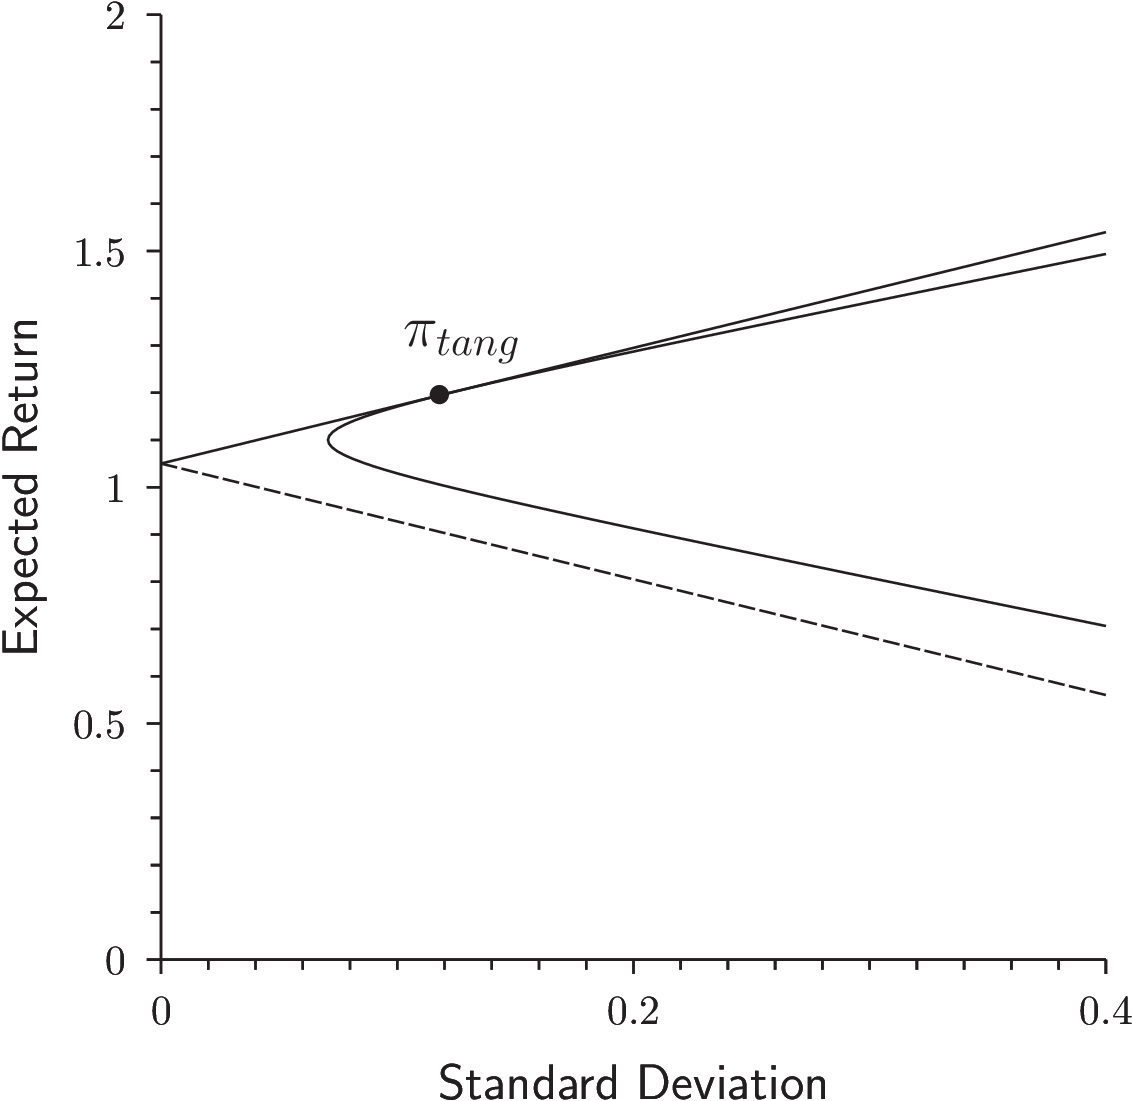
\includegraphics[scale=.7]{Images/fig5_3.png}
\end{center}
\vskip -\baselineskip
\end{frame}

\bfr\frametitle{Mean-Variance Frontier: $B/C < R_f$}
\vskip -\baselineskip
\begin{center}
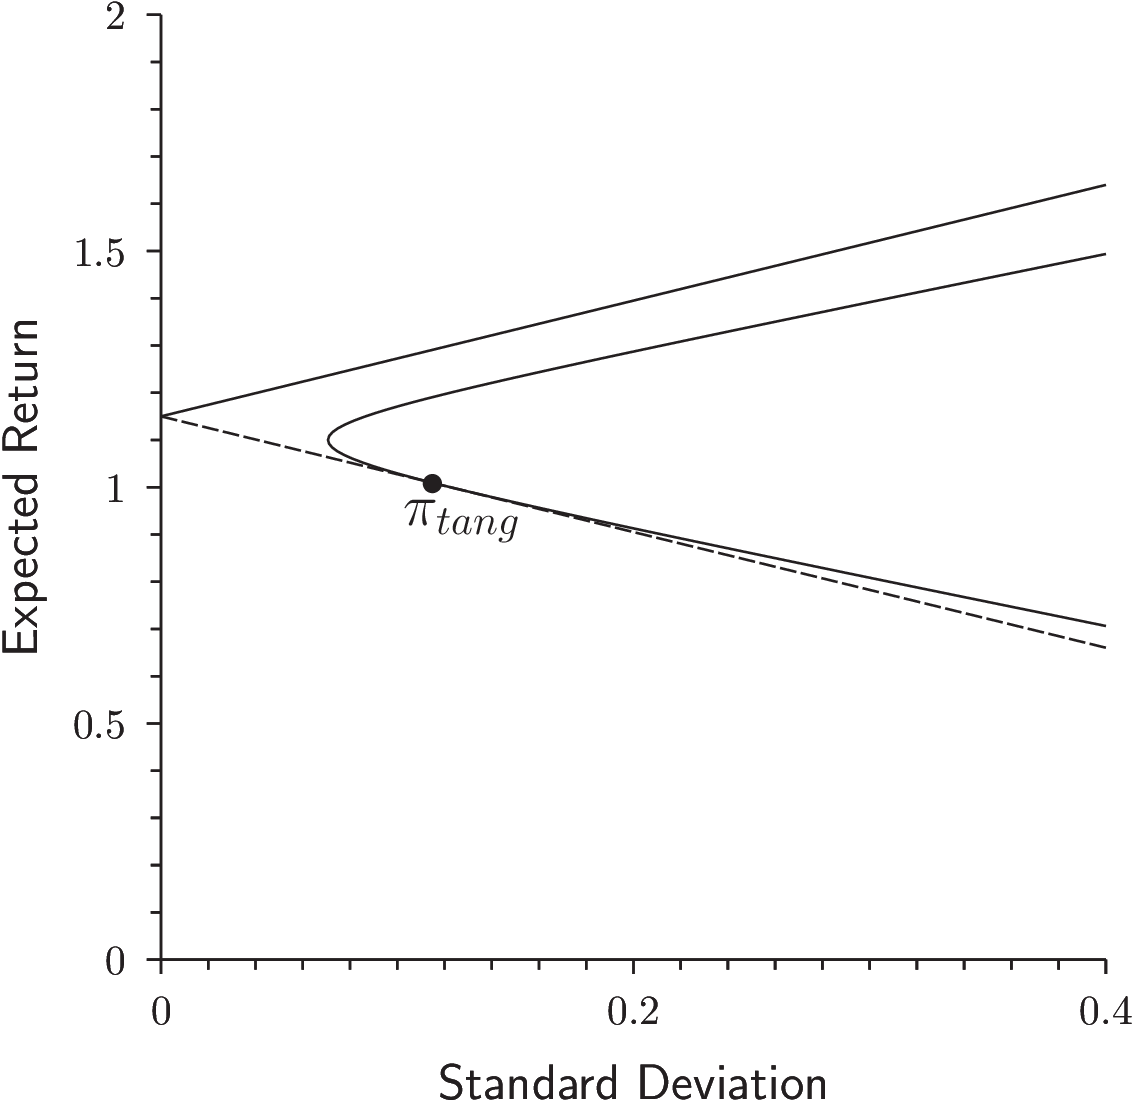
\includegraphics[scale=.7]{Images/fig5_4.png}
\end{center}
\vskip -\baselineskip
\end{frame}

\begin{frame}{What if $B/C = R_f$?}
If $B/C = R_f$, all frontier portfolios have 100\% invested in the risk-free asset and then go long and short in proportion to the positive and negative elements of $\Sigma^{-1}(\mu - R_f\iota)$.

The cone and hyperbola never touch.
\end{frame}

\bfr\frametitle{Two Fund Spanning with a Risk-Free Asset}
All frontier portfolios lie on the line through the origin and the vector $\Sigma^{-1}(\mu-R_f\iota)$ in $\myreal^n$.

Any vector on the line is a portfolio, because we are not requiring $\iota'\pi=1$.

The origin represents 100\% in the risk-free asset.

Any two portfolios on the line span the frontier in the sense that any frontier portfolio is a combination $\lambda$ and $(1-\lambda$ of the portfolios.

\end{frame}

\begin{frame}{Maximum Sharpe Ratio}
What is the risk premium of the portfolio $\Sigma^{-1}(\mu-R_f\iota)$?

What is the variance of the return of the portfolio $\Sigma^{-1}(\mu-R_f\iota)$?

What is its Sharpe ratio (risk premium divided by standard deviation)?
\end{frame}



\section{SDF}\subsection{}




\begin{frame}{Return Proportional to $\tm_p$}
Consider the SDF in the span of the assets, denoted by $\tm_p$.

This is the payoff of some portfolio (that's what it means to be in the span of the assets).

If we divide by its cost, the re-scaled payoff will have a cost of 1 and hence be a return.  Call this return $\tilde{R}_p$.  From Exercise 3.3, if there is a risk-free asset,
$$\tm_p = \frac{1}{R_f} + \left(\iota - \frac{1}{R_f}\right)\Sigma^{-1}(\tilde{\mathbf{R}} - \mu)\,.$$
This implies that $\tr_p$ is an inefficient frontier portfolio.

\end{frame}

\bfr\frametitle{HJ Bound with a Risk-Free Asset}
For any SDF $\tm$ and any return $\tr$,
$$\frac{\stdev(\tilde{m})}{\mye[\tilde{m}]}\geq  \frac{\stdev(\tilde{m}_p)}{\mye[\tilde{m}_p]} \geq  \frac{|\mye[\tilde{R}]-R_f|}{\stdev(\tilde{R})}$$
The right-hand side is the absolute value of the Sharpe ratio of $\tr$.

The second inequality is an equality for the maximum Sharpe ratio.  In fact, $$ \frac{\stdev(\tilde{m}_p)}{\mye[\tilde{m}_p]} = \frac{|\mye[\tilde{R}_p]-R_f|}{\stdev(\tilde{R}_p)}$$

\end{frame}

\section{Risk Premia}\subsection{}

\bfr\frametitle{The FOC with a Risk-Free Asset}
The FOC for the frontier with a risk-free asset is
$$\Sigma\pi \ = \ \delta (\mu-R_f\iota )$$
We solved it for $\pi$:
$$ \pi \ = \ \delta\Sigma^{-1}(\mu-R_f\iota )$$
We can instead solve it for the vector of risk premia:
$$\mu - R_f\iota \ = \ \frac{1}{\delta}\Sigma\pi$$
 What is $\Sigma \pi$?
\end{frame}



\end{document}

